% Pacotes que  fazem o sistema pegar, eh como o import do python
\documentclass[a4paper, 12pt]{article}
\usepackage[utf8]{inputenc}
\usepackage{amsmath}
\usepackage{cite}
\usepackage{indentfirst}
\usepackage{graphicx}
\usepackage[colorinlistoftodos]{todonotes}
\usepackage{tikz}
\usepackage{url}
\usepackage{enumerate}
\usepackage{float}
\usepackage{ragged2e}
\usetikzlibrary{babel}
\usetikzlibrary{calc,patterns,angles,quotes}

%Usage: \btable{table specs}{caption}{reference label}



\begin{document} %Comeco do documento

\begin{titlepage} 

\begin{figure}[H]
\centering

\includegraphics[width=1.75cm]{IFSC_USP.png} % Nome da Imagem 

\end{figure}
    \begin{center}
        Universidade de São Paulo \\
        
        Instituto de Física de São Carlos \\


\vspace{10pt}

        
        \vspace{85pt}
        
        
         \large\textbf{{Prática 1: Complexidade}} % Titulo da Pratica 
        \vspace{160pt}
        
    \end{center}
    
    \begin{flushright}
        
        Stefan Taiguara Couperus Leal 10414866
    \end{flushright}
    
    \begin{center}
        \vspace{\fill}
        02 de Agosto de 2019 % Onde eu coloco a data
    \end{center}
\end{titlepage}

\newpage

\tableofcontents    % Posso ativar para ter a tabela de conteudo

%\listoffigures

%\listoftables

\thispagestyle{empty}

\newpage
\pagenumbering{arabic}

%% Notas sobre a correção dos relatórios:
% i) Explicitar o número de medidas efetuadas; ii) Explicitar a precisão dos instrumentos na seção
% dos materiais empregados; iii) Discutir, nos resultados, qual dos métodos gerou o melhor
% resultado, o mais preciso, e indicar possíveis fontes de diferença entre os métodos empregados 
% que tenham levado às diferenças de precisão observadas;

\justifying

\section{Programas sem a otimização}

A primeira parte do experimento os programas foram rodados sem a utilização da otimização que o compilar possui, com isso os gráficos foram: 


%Como colocar figuras
\begin{figure}[H]
\centering
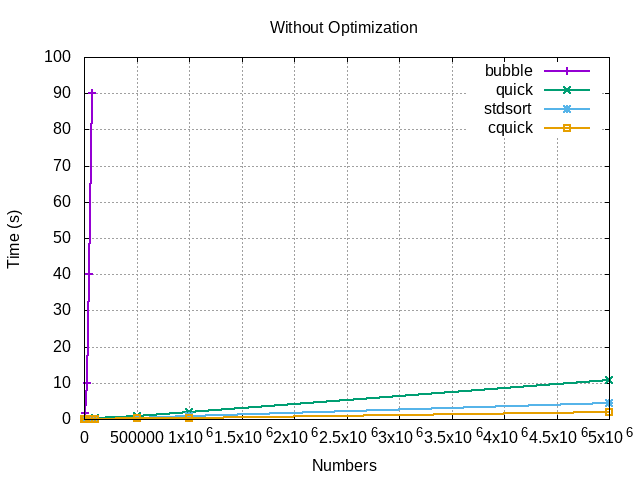
\includegraphics[width=10.0cm]{withoutOptimization.png}
\caption{}{Comparação de tempo de execução para cada método de sort sem a utilização de otimização}  
\end{figure}

\hspace{1.5cm}

Colocando na escala logarítmica.
 
%Como colocar figuras
\begin{figure}[H]
\centering
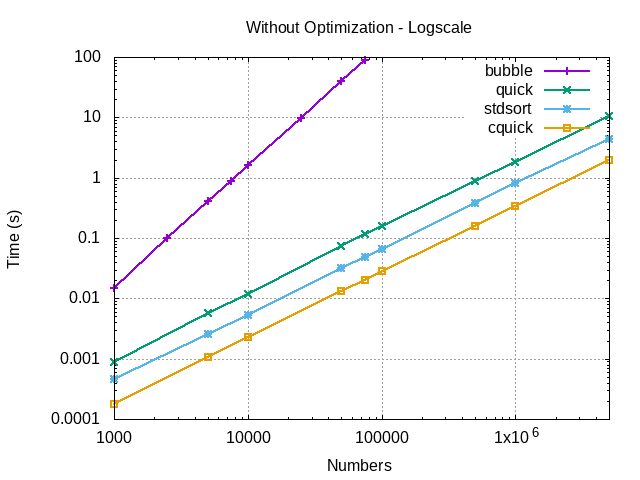
\includegraphics[width=10.0cm]{withoutOptimization_log.png}
\caption{}{Comparação de tempo de execução para cada método de sort sem a utilização de otimização}
\label{fig:without_otimization}  
\end{figure}


\vspace{0.75cm} % So para deixar um espaco maior entre os 

\section{Programas com a otimização}

Já nesta parte foi utilizado a otimização que o compilador possui, e com isso os gráficos gerados foram:

%Como colocar figuras
\begin{figure}[H]
	\centering
	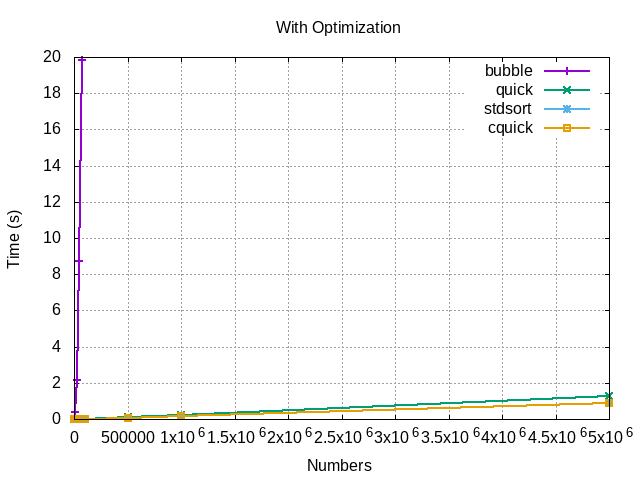
\includegraphics[width=10.0cm]{withOptimization.png}
\end{figure}

Colocando, novamente, na escala logarítmica.

%Como colocar figuras
\begin{figure}[H]
	\centering
	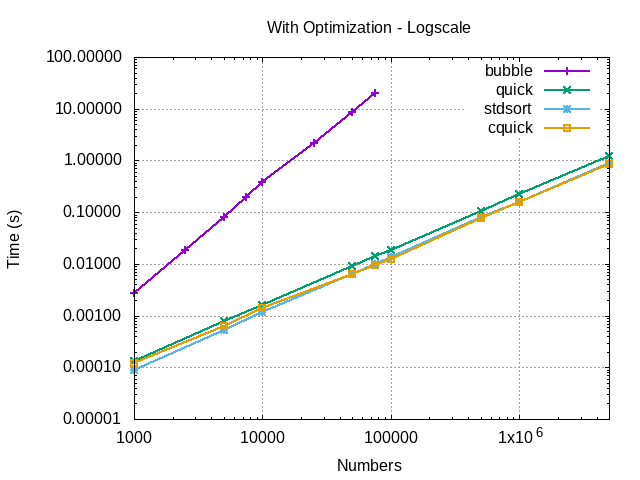
\includegraphics[width=10.0cm]{withOptimization_log.png}
\end{figure}


\section{Otimizações vistas individualmentes}

\subsection{Bubble Sort}
%Como colocar figuras
\begin{figure}[H]
	\centering
	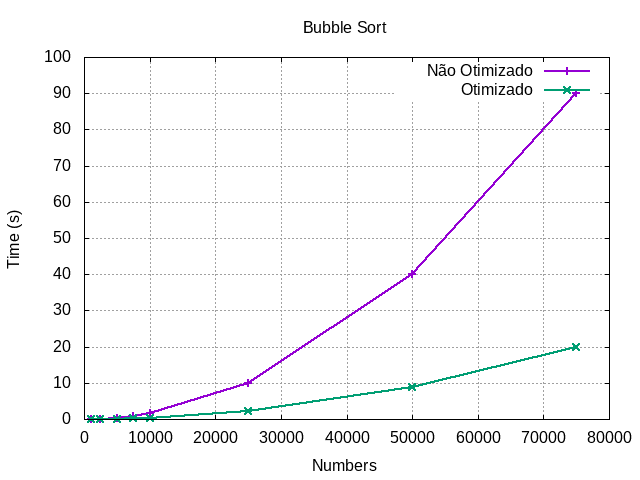
\includegraphics[width=10.0cm]{bubble.png}
\end{figure}



\begin{figure}[H]
	\centering
	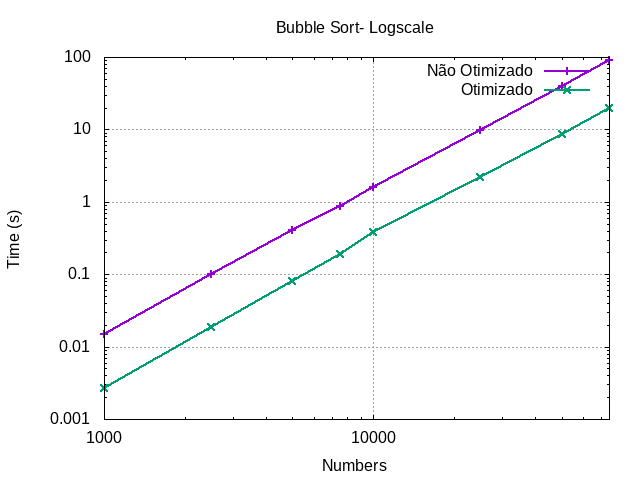
\includegraphics[width=10.0cm]{bubble_log.png}
\end{figure}



\begin{table}[H]%Como fazer uma tabela
	
	\begin{center}
		\scalebox{0.9}{
			\begin{tabular}{  l | l | l | l  }
				\label{tab:Bubble_diferenca}
				bubble.cpp & Nao otimizado & Otimizado & Diferenca \\ \hline
				N & t(s) & t(s) & \% \\ \hline
				1000 & 0.0150798 & 0.0026974 & 559.04945503077 \\ \hline
				2500 & 0.100568 & 0.0188995 & 532.119897351782 \\ \hline
				5000 & 0.403481 & 0.0815709 & 494.638406588624 \\ \hline
				7500 & 0.874547 & 0.192306 & 454.768441962289 \\ \hline
				10000 & 1.60068 & 0.38566 & 415.049525488772 \\ \hline
				25000 & 9.89544 & 2.17505 & 454.952299947128 \\ \hline
				50000 & 40.173 & 8.75064 & 459.086421107485 \\ \hline
				75000 & 90.0311 & 19.822 & 454.197860962567 \\ 
			\end{tabular}
		}
	\end{center}
	\caption{Comparação entre o uso do bubble sort com e sem a otimização}
\end{table}


Sendo a média de desempenho entre o uso ou não da otimização de:


\begin{equation*}
	M = (480 \pm 80) \%
\end{equation*}

\subsection{Quick Sort}
%Como colocar figuras

\begin{figure}[H]
	\centering
	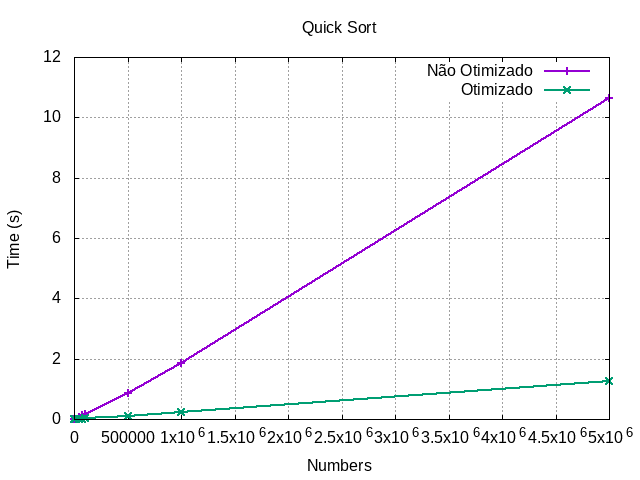
\includegraphics[width=10.0cm]{quick.png}
\end{figure}


\begin{figure}[H]
	\centering
	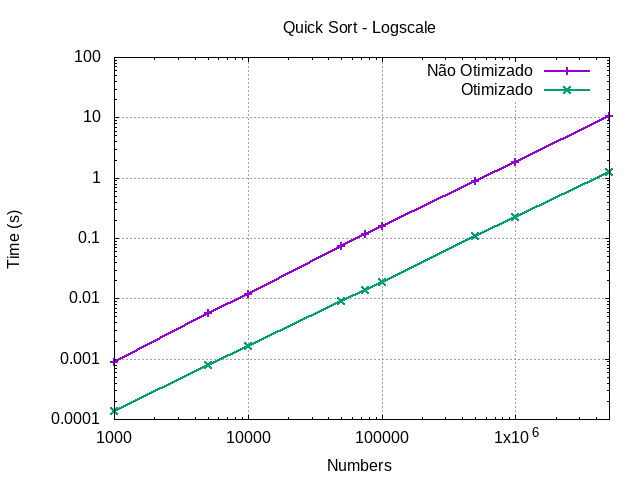
\includegraphics[width=10.0cm]{quick_log.png}
\end{figure}




\begin{table}[H] %Como fazer uma tabela
	\begin{center}
		\scalebox{0.9}{
			\begin{tabular}{  l | l | l | l  }
				quick.cpp & Não Otimizado & Otimizado & Diferença \\ \hline
				N & t(s) & t(s) & \% \\ \hline
				1000 & 0.00088135 & 0.0001349 & 653.335804299481 \\ \hline
				5000 & 0.005691 & 0.0007757 & 733.659920072193 \\ \hline
				10000 & 0.012008 & 0.00159235 & 754.105567243382 \\ \hline
				50000 & 0.0728277 & 0.00894055 & 814.577402956194 \\ \hline
				75000 & 0.117504 & 0.0139109 & 844.690135073935 \\ \hline
				100000 & 0.159358 & 0.0188964 & 843.324654431532 \\ \hline
				500000 & 0.871283 & 0.107163 & 813.044614279182 \\ \hline
				1000000 & 1.85177 & 0.225075 & 822.734644007553 \\ \hline
				5000000 & 10.6437 & 1.24485 & 855.01867694903 
			\end{tabular}
					
		}
	\end{center}
		\caption{Comparação entre o uso do quick sort com e sem a otimização}
\end{table}

Sendo a média de desempenho entre o uso ou não da otimização de:


\begin{equation*}
M = (800  \pm 70) \%
\end{equation*}


\subsection{cQuick Sort}
%Como colocar figuras
\begin{figure}[H]
	\centering
	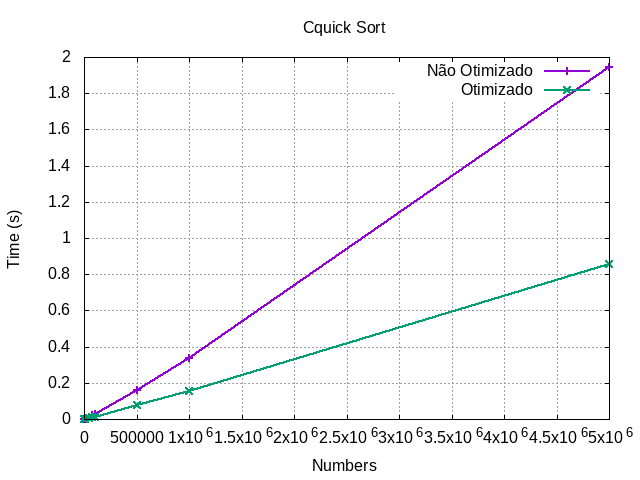
\includegraphics[width=10.0cm]{cquick.png}
\end{figure}



\begin{figure}[H]
	\centering
	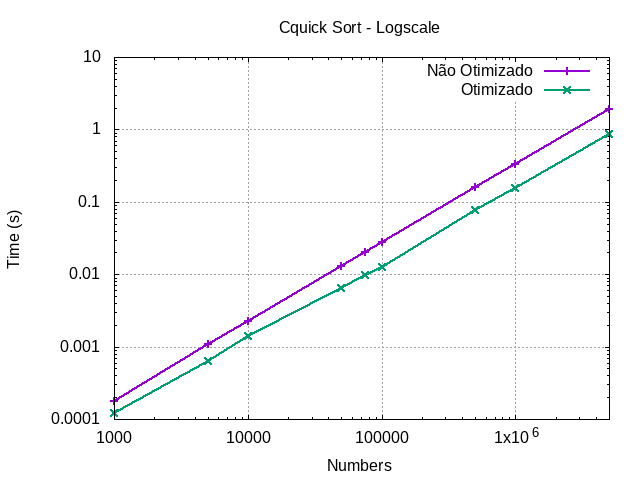
\includegraphics[width=10.0cm]{cquick_log.png}
\end{figure}



\begin{table}[H] %Como fazer uma tabela
	\begin{center}
		\scalebox{0.9}{
			\begin{tabular}{ l | l | l | l }
				cquick.cpp & Não & Otimizado & Diferença \\ \hline
				N & t(s) & t(s) & \% \\ \hline
				1000 & 0.0001796 & 0.00012165 & 147.636662556515 \\ \hline
				5000 & 0.00108565 & 0.0006263 & 173.343445633083 \\ \hline
				10000 & 0.00226915 & 0.0013973 & 162.395333858155 \\ \hline
				50000 & 0.0131055 & 0.006372 & 205.673258003766 \\ \hline
				75000 & 0.0204937 & 0.00963175 & 212.77234147481 \\ \hline
				100000 & 0.0278923 & 0.0124632 & 223.797259130881 \\ \hline
				500000 & 0.16071 & 0.0776592 & 206.942641696026 \\ \hline
				1000000 & 0.336523 & 0.156496 & 215.036167058583 \\ \hline
				5000000 & 1.94205 & 0.85818 & 226.298678598895 \\ 
			\end{tabular}
		}
	\end{center}
		\caption{Comparação entre o uso do cquick com e sem a otimização}
\end{table}


Sendo a média de desempenho entre o uso ou não da otimização de:


\begin{equation*}
M = (200 \pm 30) \%
\end{equation*}



\subsection{Stdsort}
%Como colocar figuras

\begin{figure}[H]
	\centering
	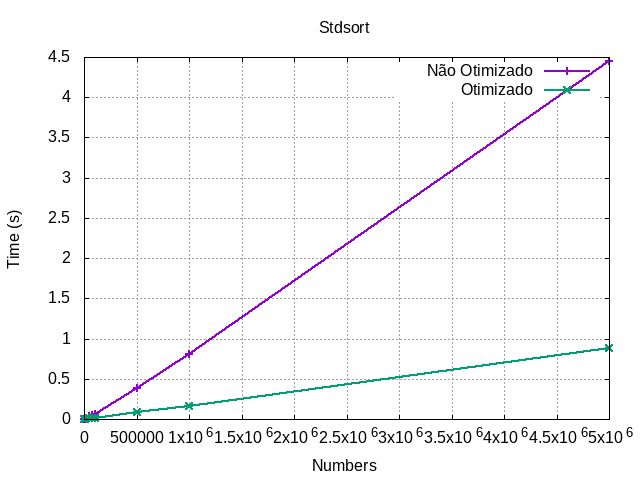
\includegraphics[width=10.0cm]{stdsort.png}
\end{figure}


\begin{figure}[H]
	\centering
	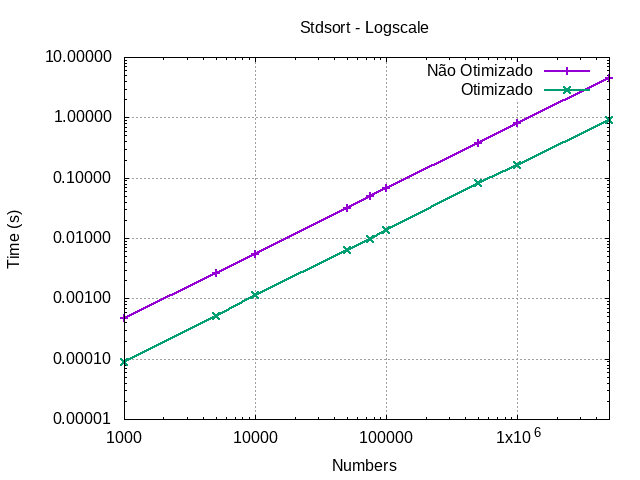
\includegraphics[width=10.0cm]{stdsort_log.png}
\end{figure}

\begin{table}[h] %Como fazer uma tabela
	\begin{center}
		\scalebox{0.9}{
			\begin{tabular}{ l | l | l | l  }
				stdsort.cpp & Não Otimizado& Otimizado & Diferença \\ \hline
				N & t(s) & t(s) & \% \\ \hline
				1000 & 0.0004638 & 8.8E-005 & 527.045454545454 \\ \hline
				5000 & 0.0025799 & 0.0005184 & 497.665895061728 \\ \hline
				10000 & 0.0053947 & 0.00114835 & 469.778377672312 \\ \hline
				50000 & 0.0313781 & 0.00631355 & 496.996143215782 \\ \hline
				75000 & 0.0488633 & 0.00975975 & 500.661389892159 \\ \hline
				100000 & 0.0664287 & 0.0133985 & 495.792066276076 \\ \hline
				500000 & 0.379537 & 0.080877 & 469.276803046602 \\ \hline
				1000000 & 0.809606 & 0.160195 & 505.387808608259 \\ \hline
				5000000 & 4.44977 & 0.888075 & 501.057906145314 \\
			\end{tabular}					
		}
	\end{center}
	\caption{Comparação entre o uso do std::sort com e sem a otimização}
\end{table}




\begin{equation*}
M = (500 \pm 20) \%
\end{equation*}



\section{Conclusão}

\textbf{Qual a complexidade de cada programa?}

\hspace{0.9cm}

\begin{table}[H] %Como fazer uma tabela
	\begin{center}
		\scalebox{0.9}{
			\begin{tabular}{c|c}
				Algoritmo & Complexidade  \\ \hline  
				bubble.cpp &  $O^2$\\  
				quick.cpp & $O (n \log n)$\\  
				cquick.cpp &  $O (n \log n)$\\  
				stdsort.cpp &  $O(n  \log n)$ \\ 
			\end{tabular} 
						
		}
	\end{center}
\end{table}



\hspace{0.9cm}

\textbf{Essa complexidade se reflete nos resultados? }

Sim, como ficou visível o bubble sort apresentou o pior resultado dentre todos, dado que sua complexidade é de $O^2$.

\textbf{O que você pode concluir sobre a importância da complexidade do programa para seu desempenho?}	

Quanto maior for a complexidade pior o desempenho que vai ser apresentado pelo programa, portanto sempre deve se ter em mente a complexidade do algoritmo utilizado.

\textbf{O que você pode concluir sobre a importância de otimizações no código?}


\begin{table}[!htp] %Como fazer uma tabela
	\begin{center}
	    
		\scalebox{0.9}{
			\begin{tabular}{c|c}
				\label{tab:referencia}
				Algoritmo & Diferença $(\%)$  \\ \hline
				bubble.cpp &  $(480 \pm 80)$\% \\ 
				quick.cpp &  $(800 \pm 70)\%$\\ 
				cquick.cpp & $(500 \pm 20)\% $ \\ 
				stdsort.cpp & $(200 \pm 30)\%$ 
			\end{tabular} 
						
		}
	\end{center}
	\caption{Tabela com as diferenças de performance quando há o uso do -O2}
\end{table}




Como pode ser visto pela tabela acima a otimização apresenta uma mudança drástica de velocidade de processamento.

\textbf{Os diversos codigo são afetados da mesma forma pelas 
otimizações?}

Como pode ser visto pela tabela citada acima percebe-se que para o stdsort.cpp a diferença foi de apenas $200\%$, mas para o quick.cpp a diferença foi de $800\%$, sendo a média para todos os algoritmos $500\%$. Conclui-se que a otimização difere para cada tipo de algoritmo.

\textbf{Como você compara o impacto da complexidade e o impacto das otimizações?}

Apesar das otimizações causarem uma diferença significativa na velocidade de processamento, ela não se equipara ao uso de métodos de complexidades inferiores.

\textbf{Para 75000 elementos, quantas vezes mais rápido é o código de ordenação do std::sort em relação bubble sort?}
 
o std::sort é 2031 vezes mais rápido do que o bubble sort para 75000 elementos. 

\textbf{Você consegue explicar a diferença entre os tempos do stdsort.cpp e do cquick.cpp otimizados?}



\begin{table}[H] %Como fazer uma tabela
	\begin{center}
		\scalebox{0.9}{
			\begin{tabular}{  l | l | l | l | l  }
				stdsort.cpp & & cquick.cpp &  & Diferença \  \\ \hline
				N & t(s) & N & t(s) & t(s)\  \\ \hline
				1000 & 8.8E-005 & 1000 & 0.00012165 & -3.365E-005 \\ \hline
				5000 & 0.0005184 & 5000 & 0.0006263 & -0.0001079 \\ \hline
				10000 & 0.00114835 & 10000 & 0.0013973 & -0.00024895 \\ \hline
				50000 & 0.00631355 & 50000 & 0.006372 & -5.84499999999998E-005 \\ \hline
				75000 & 0.00975975 & 75000 & 0.00963175 & 0.000128000000000001 \\ \hline
				100000 & 0.0133985 & 100000 & 0.0124632 & 0.0009353 \\ \hline
				500000 & 0.080877 & 500000 & 0.0776592 & 0.00321779999999999 \\ \hline
				1000000 & 0.160195 & 1000000 & 0.156496 & 0.00369900000000001 \\ \hline
				5000000 & 0.888075 & 5000000 & 0.85818 &
			\end{tabular}		
		}
	\end{center}
	\caption{}
\end{table}






Portanto conclui-se que não há uma diferença significativa de tempo entre os dois métodos utilizados, dado que a diferença média deu:

\begin{equation*}
M = (0.000	\pm 0.010)s
\end{equation*}


\textbf{Comparando quick.cpp e stdsort.cpp, você recomenda o uso de algoritmos da STL?}

\begin{figure}[H]
	\centering
	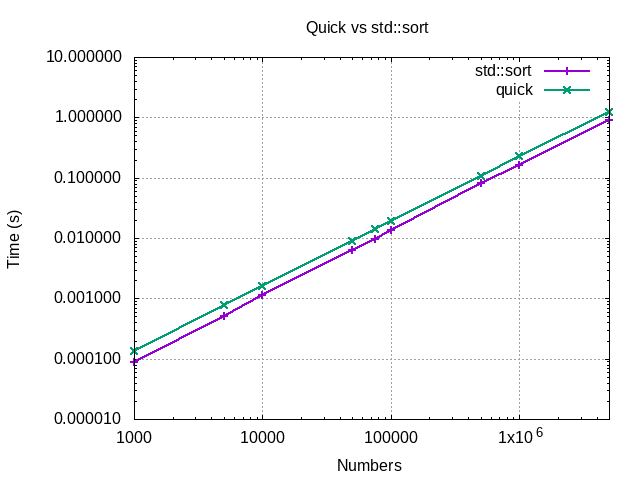
\includegraphics[width=10.0cm]{quick_vs_stdsort.png}
	\caption{}{Gráfico de Quick sort vs std::sort}
	\label{fig:quick_vs_std}  
\end{figure}

\begin{table}[H] %Como fazer uma tabela
	\begin{center}
		\scalebox{0.9}{
	
    \begin{tabular}{  l | l | l | l | l  }
    	quick.cpp & & stdsort.cpp & & Diferença  \\
    	N & t(s) & N & t(s) & \% \\ \hline
    	1000 & 0.0001349 & 1000 & 8.8E-005 & 4.69E-005 \\ \hline
    	5000 & 0.0007757 & 5000 & 0.0005184 & 0.0002573 \\ \hline
    	10000 & 0.00159235 & 10000 & 0.00114835 & 0.000444 \\ \hline
    	50000 & 0.00894055 & 50000 & 0.00631355 & 0.002627 \\ \hline
    	75000 & 0.0139109 & 75000 & 0.00975975 & 0.00415115 \\ \hline
    	100000 & 0.0188964 & 100000 & 0.0133985 & 0.0054979 \\ \hline
    	500000 & 0.107163 & 500000 & 0.080877 & 0.026286 \\ \hline
    	1000000 & 0.225075 & 1000000 & 0.160195 & 0.06488 \\ \hline
    	5000000 & 1.24485 & 5000000 & 0.888075 & 0.356775 \\ 
    \end{tabular}
    }
    	\end{center}
\end{table}


Ambos apresentam excelente tempos de execução, portanto é recomendado sim o uso de algoritmos da STL. 

\end{document}